\documentclass[tikz,border=20pt]{standalone}
\usetikzlibrary{calc,arrows.meta}
\usepackage{xcolor}

\definecolor{skinflsh}{HTML}{FCD5CE}
\definecolor{motherpink}{HTML}{F472B6}
\definecolor{motherskirt}{HTML}{0F766E}
\definecolor{sonshirt}{HTML}{EAB308}
\definecolor{vrblue}{HTML}{38BDF8}
\definecolor{woodshelf}{HTML}{A16207}

\begin{document}
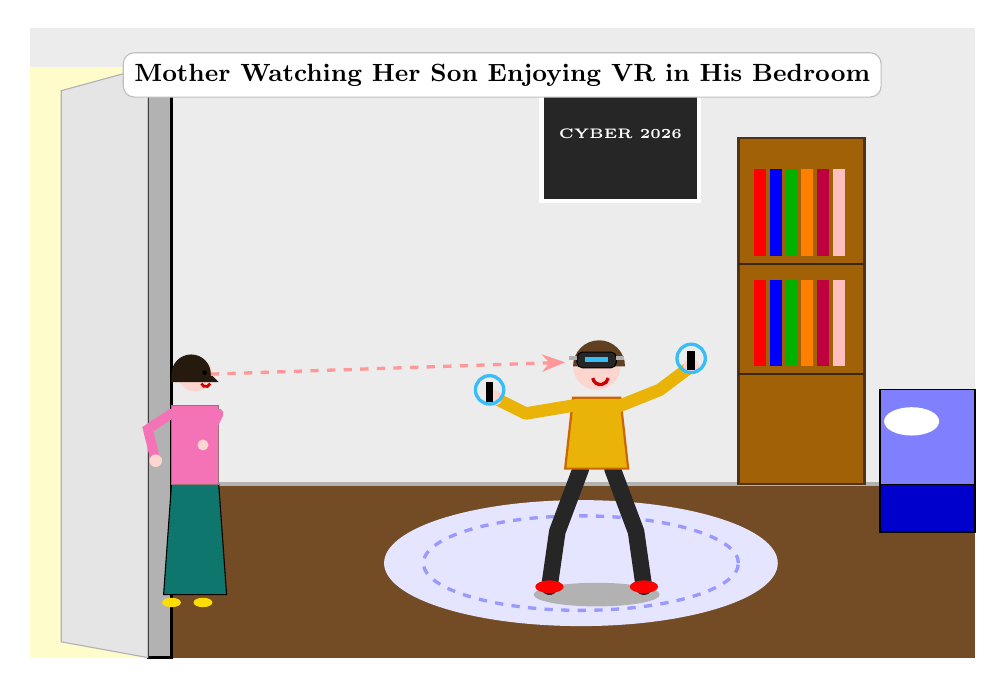
\begin{tikzpicture}[x=1cm, y=1cm, >=Stealth]

  % Room Canvas (Wall & Floor)
  \fill[gray!15] (-6, -4) rectangle (6, 4);
  \fill[brown!60!black] (-6, -4) rectangle (6, -1.8);
  \draw[gray!60, line width=1.5pt] (-6, -1.8) -- (6, -1.8);

  % ==================== FURNITURE ====================
  % 1. Wall Poster
  \filldraw[fill=black!85, draw=white, line width=1.5pt] (0.5, 1.8) rectangle (2.5, 3.5);
  \node[font=\bfseries\tiny, text=white] at (1.5, 2.65) {CYBER 2026};

  % 2. Bookshelf (Right-center)
  \filldraw[fill=woodshelf, draw=brown!40!black, thick] (3.0, -1.8) rectangle (4.6, 2.6);
  \foreach \y in {-0.4, 1.0} {
    \draw[brown!30!black, thick] (3.0, \y) -- (4.6, \y);
  }
  % Books
  \foreach \x/\c in {3.2/red, 3.4/blue, 3.6/green!70!black, 3.8/orange, 4.0/purple, 4.2/pink} {
    \fill[\c] (\x, 1.1) rectangle (\x+0.15, 2.2);
    \fill[\c] (\x, -0.3) rectangle (\x+0.15, 0.8);
  }

  % 3. Bed (Far Right)
  \filldraw[fill=blue!80!black, draw=black, thick] (4.8, -2.4) rectangle (6.0, -0.6);
  \filldraw[fill=blue!50, draw=black] (4.8, -1.8) rectangle (6.0, -0.6);
  \fill[white] (5.2, -1.0) ellipse (0.35 and 0.18);

  % Circular Play Mat Rug
  \fill[blue!10] (1.0, -2.8) ellipse (2.5 and 0.8);
  \draw[blue!40, dashed, line width=1.2pt] (1.0, -2.8) ellipse (2.0 and 0.6);

  % ==================== SON PLAYING VR (Center: (1.2, -1.5)) ====================
  % Floor Shadow
  \fill[black!30] (1.2, -3.2) ellipse (0.8 and 0.15);

  % Dynamic Legs (bent knees)
  \draw[black!85, line width=6pt, line cap=round, line join=round]
    (1.0, -1.6) -- (0.7, -2.4) -- (0.6, -3.1);
  \fill[red] (0.6, -3.1) ellipse (0.18 and 0.08);

  \draw[black!85, line width=6pt, line cap=round, line join=round]
    (1.4, -1.6) -- (1.7, -2.4) -- (1.8, -3.1);
  \fill[red] (1.8, -3.1) ellipse (0.18 and 0.08);

  % Torso (Yellow T-shirt)
  \filldraw[fill=sonshirt, draw=orange!80!black, thick]
    (0.8, -1.6) -- (1.6, -1.6) -- (1.5, -0.7) -- (0.9, -0.7) -- cycle;

  % Arms with VR Controllers
  % Left Arm (stretching left)
  \draw[sonshirt, line width=4.5pt, line cap=round, line join=round]
    (0.9, -0.8) -- (0.3, -0.9) -- (-0.1, -0.7);
  \fill[skinflsh] (-0.1, -0.7) circle (0.1);
  % Controller & Ring
  \fill[black] (-0.2, -0.75) rectangle (-0.12, -0.5);
  \draw[vrblue, line width=1.2pt] (-0.16, -0.6) circle (0.18);

  % Right Arm (reaching high right)
  \draw[sonshirt, line width=4.5pt, line cap=round, line join=round]
    (1.5, -0.8) -- (2.0, -0.6) -- (2.4, -0.3);
  \fill[skinflsh] (2.4, -0.3) circle (0.1);
  % Controller & Ring
  \fill[black] (2.35, -0.35) rectangle (2.45, -0.1);
  \draw[vrblue, line width=1.2pt] (2.4, -0.2) circle (0.18);

  % Head & Hair
  \fill[skinflsh] (1.2, -0.3) circle (0.3);
  \fill[brown!50!black] (0.9, -0.3) arc (180:0:0.33) -- cycle;
  % Excited smile
  \draw[red!80!black, line width=1.2pt] (1.15, -0.45) arc (190:350:0.1);

  % VR Goggles / Headset
  \filldraw[fill=black!85, draw=black, rounded corners=2pt] (0.95, -0.32) rectangle (1.45, -0.12);
  \fill[vrblue] (1.05, -0.24) rectangle (1.35, -0.18);
  \draw[gray!60, line width=1.5pt] (0.95, -0.2) -- (0.85, -0.2);
  \draw[gray!60, line width=1.5pt] (1.45, -0.2) -- (1.55, -0.2);


  % ==================== MOTHER AT DOORWAY (Left: (-4.5, -1.5)) ====================
  % Hallway / Open Door
  \fill[yellow!20] (-6, -4) rectangle (-4.5, 3.5);
  \filldraw[fill=gray!60, draw=black, thick] (-4.5, -4) rectangle (-4.2, 3.5);
  % Open door leaf
  \filldraw[fill=gray!20, draw=gray!60] (-5.6, -3.8) -- (-4.5, -4) -- (-4.5, 3.5) -- (-5.6, 3.2) -- cycle;

  % Mother
  % Skirt
  \filldraw[fill=motherskirt, draw=black] (-4.2, -1.8) -- (-3.6, -1.8) -- (-3.5, -3.2) -- (-4.3, -3.2) -- cycle;
  \fill[yellow!80!orange] (-4.2, -3.3) ellipse (0.12 and 0.06);
  \fill[yellow!80!orange] (-3.8, -3.3) ellipse (0.12 and 0.06);

  % Cardigan / Blouse
  \filldraw[fill=motherpink, draw=pink!60!black] (-4.2, -1.8) -- (-3.6, -1.8) -- (-3.6, -0.8) -- (-4.2, -0.8) -- cycle;

  % Arms: Left leaning on door frame, right hand on heart
  \draw[motherpink, line width=3.5pt, line cap=round] (-4.2, -0.9) -- (-4.5, -1.1) -- (-4.4, -1.5);
  \fill[skinflsh] (-4.4, -1.5) circle (0.08);

  \draw[motherpink, line width=3.5pt, line cap=round] (-3.6, -0.9) -- (-3.8, -1.3);
  \fill[skinflsh] (-3.8, -1.3) circle (0.07);

  % Head & Hair
  \fill[skinflsh] (-3.9, -0.4) circle (0.22);
  \fill[black!80!brown] (-4.2, -0.4) arc (180:0:0.25) -- (-3.6, -0.5) -- (-4.2, -0.5) -- cycle;
  % Eye looking right & warm smile
  \fill[black] (-3.78, -0.38) circle (0.03);
  \draw[red!80!black, line width=1pt] (-3.82, -0.52) arc (200:340:0.06);

  % Affectionate sightline from Mother to Son
  \draw[pink!80!red, dashed, line width=1.2pt, ->] (-3.7, -0.4) -- (0.8, -0.25);

  % Title note
  \node[draw=gray!50, fill=white, rounded corners=4pt, font=\bfseries\small, inner sep=4pt] at (0, 3.4) {
    Mother Watching Her Son Enjoying VR in His Bedroom
  };

\end{tikzpicture}
\end{document}
